\documentclass[border=10pt]{standalone}
\usepackage{tikz,amsmath}
\usetikzlibrary{arrows.meta}

\definecolor{ub}{RGB}{114,150,200}
\definecolor{ubl}{RGB}{40,80,140}
\colorlet{cblue}{blue!50!black}
\colorlet{cred}{red!50!black}
\colorlet{cgreen}{green!50!black}
\colorlet{cgray}{gray!60}
\colorlet{cteal}{teal!70!black}

\begin{document}
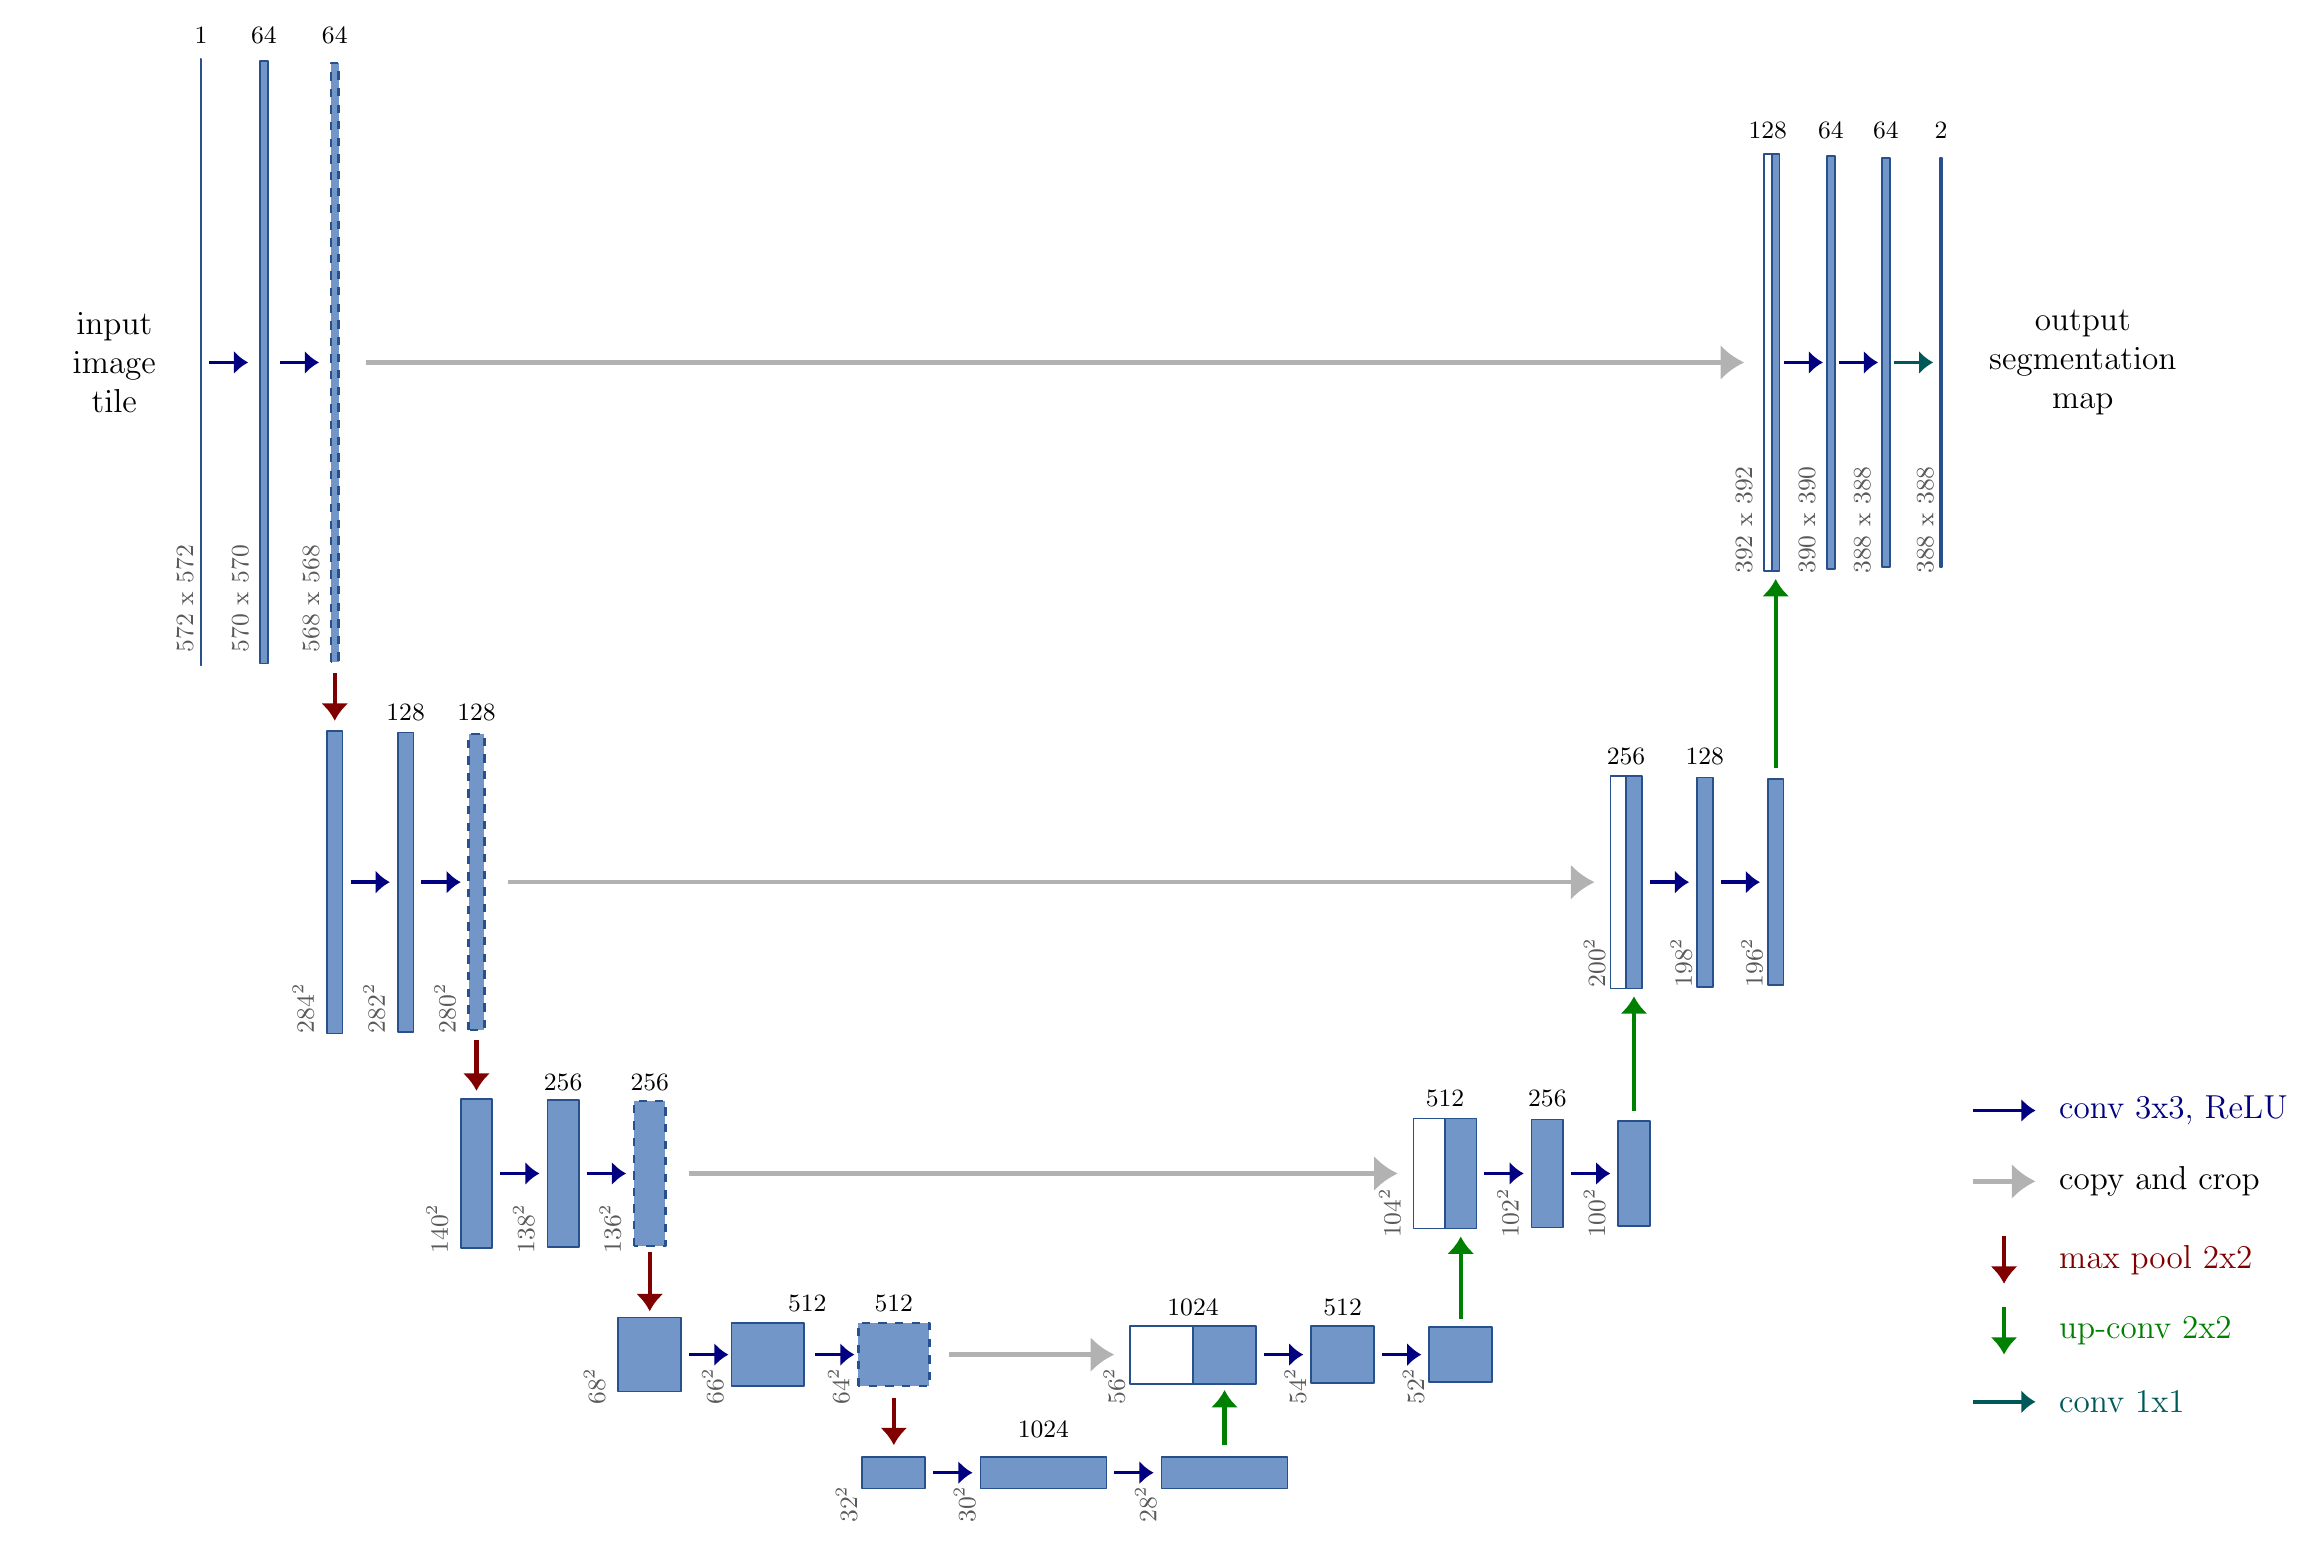
\begin{tikzpicture}[
    font=\small, line join=round,
    every node/.style={inner sep=0pt, outer sep=0pt, align=center},
    box/.style={draw=ubl, fill=ub, line width=.6pt},
    boxd/.style={draw=ubl, fill=ub, line width=.9pt, dashed},
    wbox/.style={draw=ubl, fill=white, line width=.6pt},
    sz/.style={rotate=90, text=gray!70!black, font=\small},
    % ===== 箭头优化：头变小、线加粗，线身可见 =====
    barr/.style={cblue, line width=1.2pt, -{Latex[length=1.8mm, width=3mm]}},
    marr/.style={cred, line width=1.6pt, -{Latex[length=2.2mm, width=3.5mm]}},
    uarr/.style={cgreen, line width=1.6pt, -{Latex[length=2.2mm, width=3.5mm]}},
    garr/.style={cgray, line width=1.6pt, -{Latex[length=3mm, width=4.5mm]}},
    tarr/.style={cteal, line width=1.2pt, -{Latex[length=1.8mm, width=3mm]}}
  ]

  % ========== 宏 ==========
  \newcommand{\vbx}[4]{\draw[box] ({#1-#4/2},{#2-#3/2}) rectangle ++(#4,#3);}
  \newcommand{\vbxD}[4]{\draw[boxd] ({#1-#4/2},{#2-#3/2}) rectangle ++(#4,#3);}
  \newcommand{\hbx}[4]{\draw[box] ({#1-#3/2},{#2-#4/2}) rectangle ++(#3,#4);}
  \newcommand{\hbxD}[4]{\draw[boxd] ({#1-#3/2},{#2-#4/2}) rectangle ++(#3,#4);}

  % ========== 左 A 层 ==========
  \vbx{1.0}{10}{7.7}{.01}            \node at (1.0,14.15) {1};
  \node[sz] at (0.8,7) {572 x 572};
  \draw[barr] (1.1,10) -- (1.6,10);
  \vbx{1.8}{10}{7.65}{.1}            \node at (1.8,14.15) {64};
  \node[sz] at (1.5,7) {570 x 570};
  \draw[barr] (2.0,10) -- (2.5,10);
  \vbxD{2.7}{10}{7.6}{.1}            \node at (2.7,14.15) {64};
  \node[sz] at (2.4,7) {568 x 568};

  % ========== 左 B 层 ==========
  \draw[marr] (2.7,6.05) -- (2.7,5.45);
  \vbx{2.7}{3.4}{3.84}{.2};
  \node[sz] at (2.3,1.8) {284\textsuperscript{2}};
  \draw[barr] (2.9,3.4) -- (3.4,3.4);
  \vbx{3.6}{3.4}{3.8}{.2}           \node at (3.6,5.55) {128};
  \node[sz] at (3.2,1.8) {282\textsuperscript{2}};
  \draw[barr] (3.8,3.4) -- (4.3,3.4);
  \vbxD{4.5}{3.4}{3.76}{.2}         \node at (4.5,5.55) {128};
  \node[sz] at (4.1,1.8) {280\textsuperscript{2}};

  % ========== 左 C 层 ==========
  \draw[marr] (4.5,1.4) -- (4.5,0.75);
  \vbx{4.5}{-0.3}{1.90}{.4};
  \node[sz] at (4.0,-1.0) {140\textsuperscript{2}};
  \draw[barr] (4.8,-0.3) -- (5.3,-0.3);
  \vbx{5.6}{-0.3}{1.87}{.4}          \node at (5.6,0.85) {256};
  \node[sz] at (5.1,-1.0) {138\textsuperscript{2}};
  \draw[barr] (5.9,-0.3) -- (6.4,-0.3);
  \vbxD{6.7}{-0.3}{1.84}{.4}         \node at (6.7,0.85) {256};
  \node[sz] at (6.2,-1.0) {136\textsuperscript{2}};

  % ========== 左 D 层 ==========
  \draw[marr] (6.7,-1.3) -- (6.7,-2.05);
  \vbx{6.7}{-2.6}{.94}{.8};
  \node[sz] at (6.0,-3.0) {68\textsuperscript{2}};
  \draw[barr] (7.2,-2.6) -- (7.7,-2.6);
  \hbx{8.2}{-2.6}{.92}{.8}           \node at (8.7,-1.95) {512};
  \node[sz] at (7.5,-3.0) {66\textsuperscript{2}};
  \draw[barr] (8.8,-2.6) -- (9.3,-2.6);
  \hbxD{9.8}{-2.6}{.9}{.8}         \node at (9.8,-1.95) {512};
  \node[sz] at (9.1,-3.0) {64\textsuperscript{2}};

  % ========== 底部 ==========
  \draw[marr] (9.8,-3.15) -- (9.8,-3.75);
  \hbx{9.8}{-4.1}{.8}{.4}
  \node[sz] at (9.2,-4.5) {32\textsuperscript{2}};
  \draw[barr] (10.3,-4.1) -- (10.8,-4.1);
  \hbx{11.7}{-4.1}{1.6}{.4}         \node at (11.7,-3.55) {1024};
  \node[sz] at (10.7,-4.5) {30\textsuperscript{2}};
  \draw[barr] (12.6,-4.1) -- (13.1,-4.1);
  \hbx{14.0}{-4.1}{1.6}{.4}
  \node[sz] at (13.0,-4.5) {28\textsuperscript{2}};

  % ========== 右下行 ==========
  % 上采样箭头指向右侧蓝色上采样特征图中心，与左侧 56^2 保持充裕间隔
  \draw[uarr] (14.0,-3.75) -- (14.0,-3.05);
  \draw[garr] (10.5,-2.6) -- (12.6,-2.6);
  \draw[wbox] (12.8,-2.975) rectangle ++(.8,.74);
  \draw[box] (13.6,-2.975) rectangle ++(.8,.74);
  \node at (13.6,-2.0) {1024};
  \node[sz] at (12.6,-3.0) {56\textsuperscript{2}};
  \draw[barr] (14.5,-2.6) -- (15.0,-2.6);
  \hbx{15.5}{-2.6}{.8}{.72}          \node at (15.5,-2.0) {512};
  \node[sz] at (14.9,-3.0) {54\textsuperscript{2}};
  \draw[barr] (16.0,-2.6) -- (16.5,-2.6);
  \hbx{17.0}{-2.6}{.8}{.70}
  \node[sz] at (16.4,-3.0) {52\textsuperscript{2}};

  % ========== 右 C' 层 ==========
  \draw[uarr] (17.0,-2.15) -- (17.0,-1.1);
  \draw[garr] (7.2,-0.3) -- (16.2,-0.3);
  \draw[wbox] (16.4,-1.0) rectangle ++(.4,1.4);
  \draw[box] (16.8,-1.0) rectangle ++(.4,1.4);
  \node at (16.8,0.65) {512};
  \node[sz] at (16.1,-0.8) {104\textsuperscript{2}};
  \draw[barr] (17.3,-0.3) -- (17.8,-0.3);
  \vbx{18.1}{-0.3}{1.37}{.4}         \node at (18.1,0.65) {256};
  \node[sz] at (17.6,-0.8) {102\textsuperscript{2}};
  \draw[barr] (18.4,-0.3) -- (18.9,-0.3);
  \vbx{19.2}{-0.3}{1.34}{.4}
  \node[sz] at (18.7,-0.8) {100\textsuperscript{2}};

  % ========== 右 B' 层 ==========
  \draw[uarr] (19.2,0.5) -- (19.2,1.95);
  \draw[garr] (4.9,3.4) -- (18.7,3.4);
  \draw[wbox] (18.9,2.05) rectangle ++(.2,2.7);
  \draw[box] (19.1,2.05) rectangle ++(.2,2.7);
  \node at (19.1,5.0) {256};
  \node[sz] at (18.7,2.38) {200\textsuperscript{2}};
  \draw[barr] (19.4,3.4) -- (19.9,3.4);
  \vbx{20.1}{3.4}{2.66}{.2}         \node at (20.1,5.0) {128};
  \node[sz] at (19.8,2.38) {198\textsuperscript{2}};
  \draw[barr] (20.3,3.4) -- (20.8,3.4);
  \vbx{21.0}{3.4}{2.62}{.2}
  \node[sz] at (20.7,2.38) {196\textsuperscript{2}};

  % ========== 右 A' 层 ==========
  \draw[uarr] (21.0,4.85) -- (21.0,7.25);
  \draw[garr] (3.1,10) -- (20.6,10);
  \draw[wbox] (20.85,7.35) rectangle ++(.1,5.3);
  \draw[box] (20.95,7.35) rectangle ++(.1,5.3);
  \node at (20.9,12.95) {128};
  \node[sz] at (20.6,8) {392 x 392};
  \draw[barr] (21.1,10) -- (21.6,10);
  \vbx{21.7}{10}{5.25}{.1}           \node at (21.7,12.95) {64};
  \node[sz] at (21.4,8) {390 x 390};
  \draw[barr] (21.8,10) -- (22.3,10);
  \vbx{22.4}{10}{5.2}{.1}           \node at (22.4,12.95) {64};
  \node[sz] at (22.1,8) {388 x 388};
  \draw[tarr] (22.5,10) -- (23.0,10);
  \vbx{23.1}{10}{5.2}{.02}          \node at (23.1,12.95) {2};
  \node[sz] at (22.9,8) {388 x 388};

  % ========== 文字 ==========
  \node[text width=2.2cm, font=\large] at (-0.1,10) {input\\image\\tile};
  \node[text width=3cm, font=\large, anchor=west] at (23.4,10) {output\\segmentation\\map};

  % ========== 图例 ==========
  \draw[barr] (23.5,0.5) -- (24.3,0.5);
  \node[anchor=west, font=\large, text=cblue] at (24.6,0.5) {conv 3x3, ReLU};
  \draw[garr] (23.5,-0.4) -- (24.3,-0.4);
  \node[anchor=west, font=\large] at (24.6,-0.4) {copy and crop};
  \draw[marr] (23.9,-1.1) -- (23.9,-1.7);
  \node[anchor=west, font=\large, text=cred] at (24.6,-1.4) {max pool 2x2};
  \draw[uarr] (23.9,-2.0) -- (23.9,-2.6);
  \node[anchor=west, font=\large, text=cgreen] at (24.6,-2.3) {up-conv 2x2};
  \draw[tarr] (23.5,-3.2) -- (24.3,-3.2);
  \node[anchor=west, font=\large, text=cteal] at (24.6,-3.2) {conv 1x1};

\end{tikzpicture}
\end{document}